\section{Ergo's Native Token}
\label{sec:currency}

As most of the blockchain systems, Ergo platform have its native token which is
called \Erg{} and is divisible to up to $10^9$ smallest units, \nanoErg{}s.
\Erg{} provides stability to Ergo platform by several meaningful applications.

During the initial phase of Ergo live, miners will receive the reward in \Erg{}s created
out of thin air according to a predefined and hard-coded token emission schedule
~(see~\ref{sec:emission} for more details).
This coins will incentivize miners to participate in the Ergo network, securing it from hashrate-based attacks
like the known 51\% attack.

\Erg{} emission will be finished within just eight years, and after that miner will only receive \Erg{} from
fees.
Ergo block size and block computation cost are limited, and thus miners are enforced to
choose only a subset of transactions from mempool during high load.
Fees will help miners to sort the transactions, preventing spam attacks while allowing
to include transactions from honest users in blocks.

Besides network and computation resources, a transaction utilizes storage by increasing state size.
In existing cryptocurrencies, an element of the state once created lives possibly forever without
paying anything for that, leading to continuously increasing state size.
In contrast, Ergo has a storage rent component that periodically charges users for every byte
included in the state.
This storage rent is making the system more stable by limiting state size, returning lost coins into
circulation and providing an additional stable and predictable reward to miners.

Thus, being a platform for contractual money, Ergo is suitable to build applications and monetary systems
on top of it.
However, participating in such systems would require to use Erg, making the network more stable and secure.

\subsection{Emission}
\label{sec:emission}


All \Erg{} tokens that will ever circulate in the system are presented in the initial state and
that will consists of 3 boxes:

\begin{itemize}
    \item{\em No premine proof.} This box contains exactly one~\Erg{} and is protected by the script
    that is preventing it from spending by anyone.
    Thus, it is a long-lived box that will stay in the system until storage-rent component
    destroys it.
    Its main purpose is to prove that \Ergo{} mining was not started privately by anyone before
    the declared launch date.
    To achieve this, additional registers of this box contains latest titles from media (The Guardian, Vedomosti, Xinhua)
    as well as latest block identifiers from Bitcoin and Ethereum.
    Thus, \Ergo{} mining could not be started before certain events in the real world and the
    cryptocurrency space.

    \item{\em Treasury.} This box contain 4,330,791.5 \Erg{} that will be used to fund \Ergo{}
    development.
    Its protecting script~\cite{link to corresponding ergo tree} consists of two parts.

    First, it ensures that only a predefined portion of the box value is unlocked.
    During blocks 1-525,599 (2 years) 7.5 \Erg{} will be released every block,
    during blocks 525,600-590,399 (3 months) 4.5 \Erg{} will be released every block, and finally,
    during blocks 590,400-655,199 (3 months) 1.5 \Erg{} will be released every block.
    This rule ensures the presence of funds for \Ergo{} development for at least 2.5 years and, at any moment of time,
    rewards do not exceed 10\% of the total number of coins in circulation.

    Second, it has custom protection from unexpected spending.
    Initially, it requires that spending transaction should be signed by at least 2 of 3 secret keys
    that are under control of initial team members. When they spend the box, they are free to
    change this part of the script as they wish, for example by adding new members to protect foundation
    funds.

    During the first year, these funds are going to be used to cover pre-issued EFYT token~\cite{our website with swap },
    after that they will be distributed in a decentralized manner via a community voting system that is under development.


    \item{\em Miners reward.} This box contains 93,409,132 \Erg{} that will be collected by block miners
    as rewards for their work.
    Its protecting script~\cite{link to corresponding ergo tree} requires that spending transaction
    should have exactly two outputs with the following properties:

    \begin{itemize}
    \item{} the first output should be protected by the same script and number of \Erg{} in it should
    equal to the remaining miners' reward.
    During blocks 1 - 525,599 (2 years) miner will be able to collect 67.5 \Erg{} from this box,
    during blocks 525,600 - 590,399 (3 month) miner will be able to collect 66 \Erg{} and after
    that block reward will be reduced by 3 \Erg{} every 64,800 blocks (3 months) until it reaches zero
    at block 2,080,799.

    \item{} the second output should contain the remaining coins and should be protected by the following condition:
    it can be spent by a miner that solved the block's PoW puzzle and not earlier than 720 blocks after the current block.
    % These restrictions are done to prevent mining pools formation, see~\ref{sec:autolykos} for more details.
    \end{itemize}

\end{itemize}

All these rules results in the following curve of the number of coins in circulation with time:

\begin{figure}[H]
    \centering
    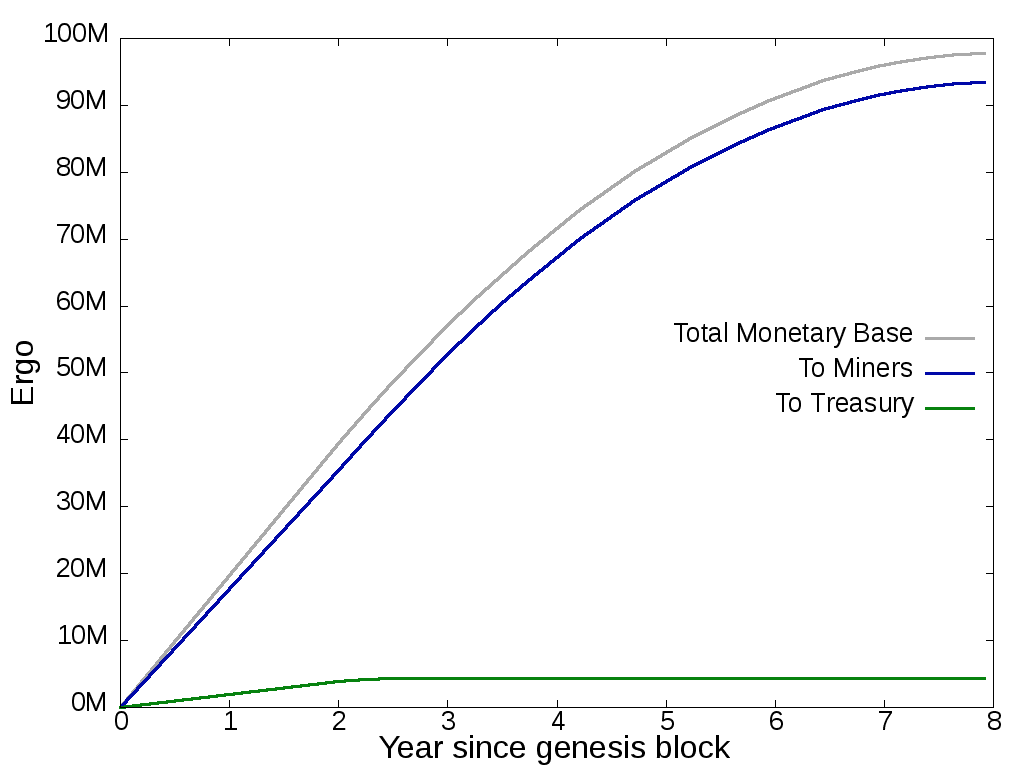
\includegraphics[width=\textwidth]{img/emission.png}
    \caption{Ergo emission curve
    \label{fig:emission} }
\end{figure}
